\subsection{Características demográficas de usuarios}

En esta sección se hará un análisis de las características demográficas de los usuarios del sistema MiBici. En particular se estudiará la distribución de edades del conjunto de todos los usuarios, la proporción de usuarios por cada género, así como las distribuciones de edades para los usuarios de género masculino y femenino por separado.

\subsubsection{Proporción de usuarios por género}

El número total de usuarios diferentes que utilizaron el sistema en el intervalo de enero de 2015 a diciembre 2018 fue $36917$ de los cuales $2$ no registraron su género. El número de usuarios de genero masculino es de $27363$ y $9552$ son de género femenino. Esto puede ser visualizado en la figura \ref{fig:genderprop}.

\begin{figure}[H]
	\centering
	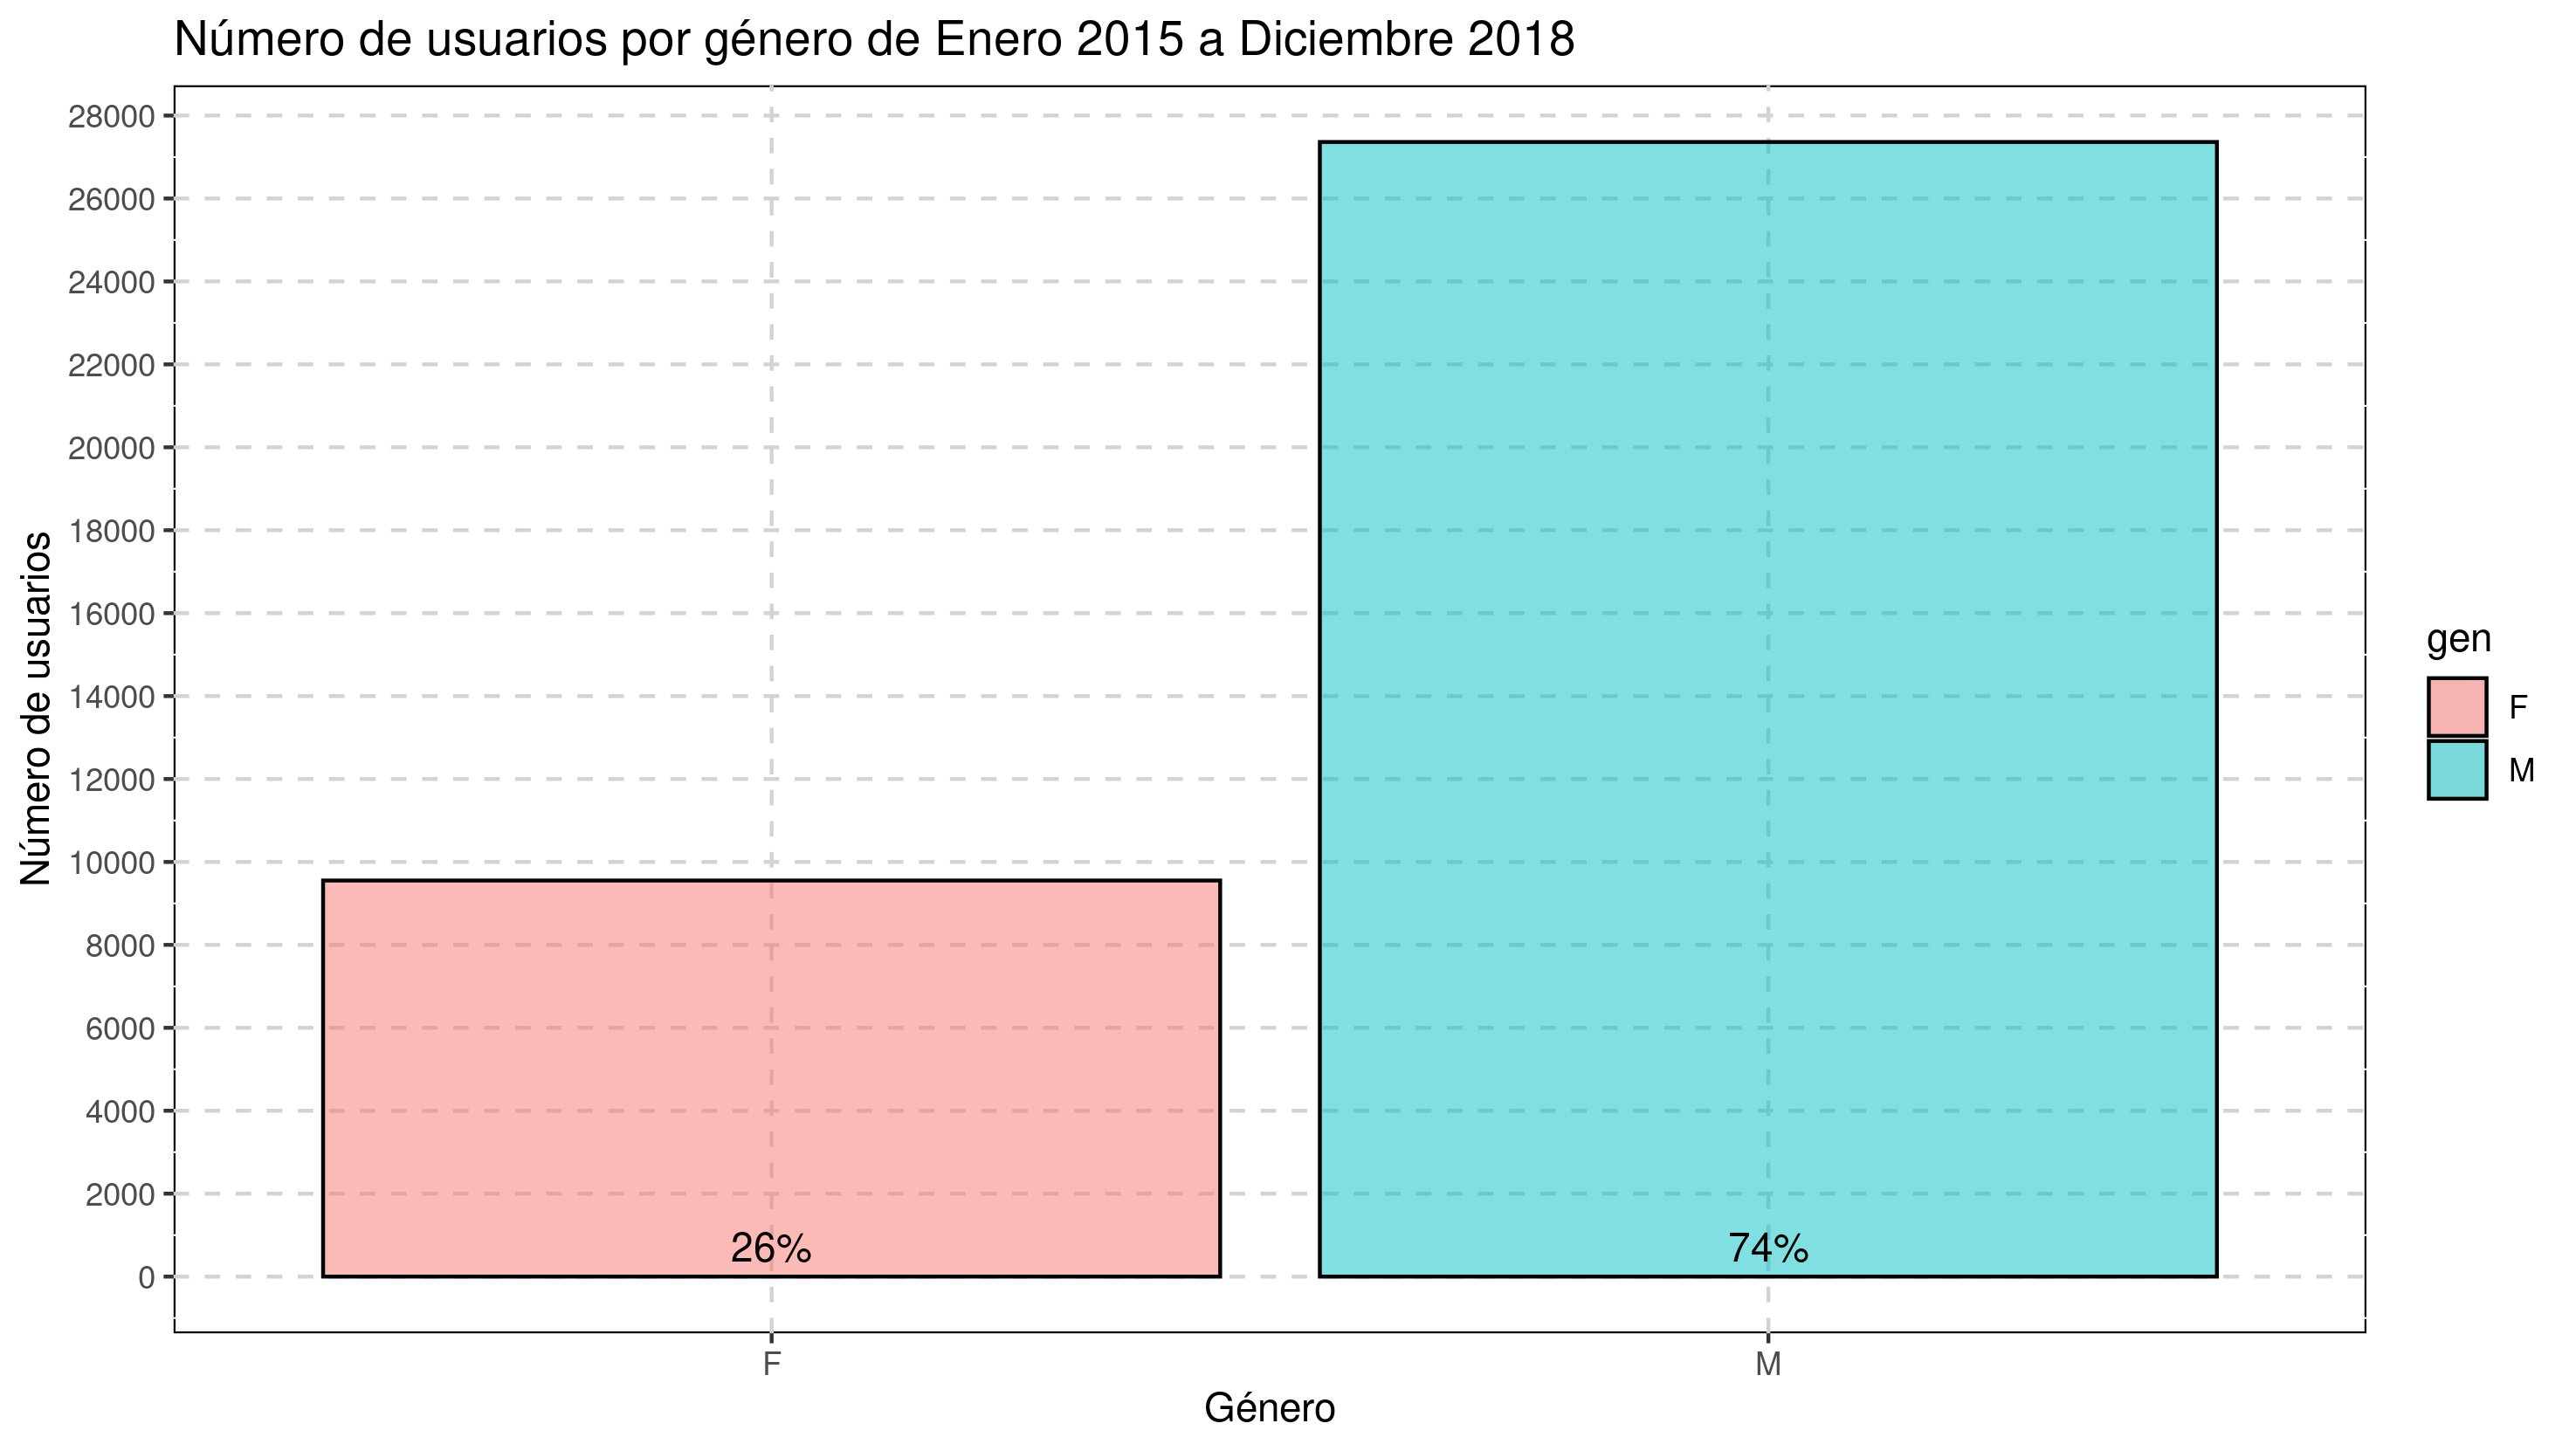
\includegraphics[width=14cm]{Graphics/genderProp}
	\caption{Número de usuarios por género de Enero 2015 a Diciembre 2018.}
	\label{fig:genderprop}
\end{figure}

En donde se puede observar que el $74\%$ de los usuarios son hombres y $26\%$ son mujeres. Se deja fuera de la gráfica a los dos usuarios que no registraron su género debido a que su contribución a las proporciones es muy pequeña.

\subsubsection*{Número de usuarios por edad}

En la figura \ref{fig:agedistribution} se puede observar la distribución de los usuarios por edades al momento de su primer registro en el sistema en el intervalo de 2015 a 2018. Para la realización de esta figura se tomó en cuenta solo la primera aparición de todos los usuarios distintos en ese intervalo de tiempo.

\begin{figure}[H]
	\centering
	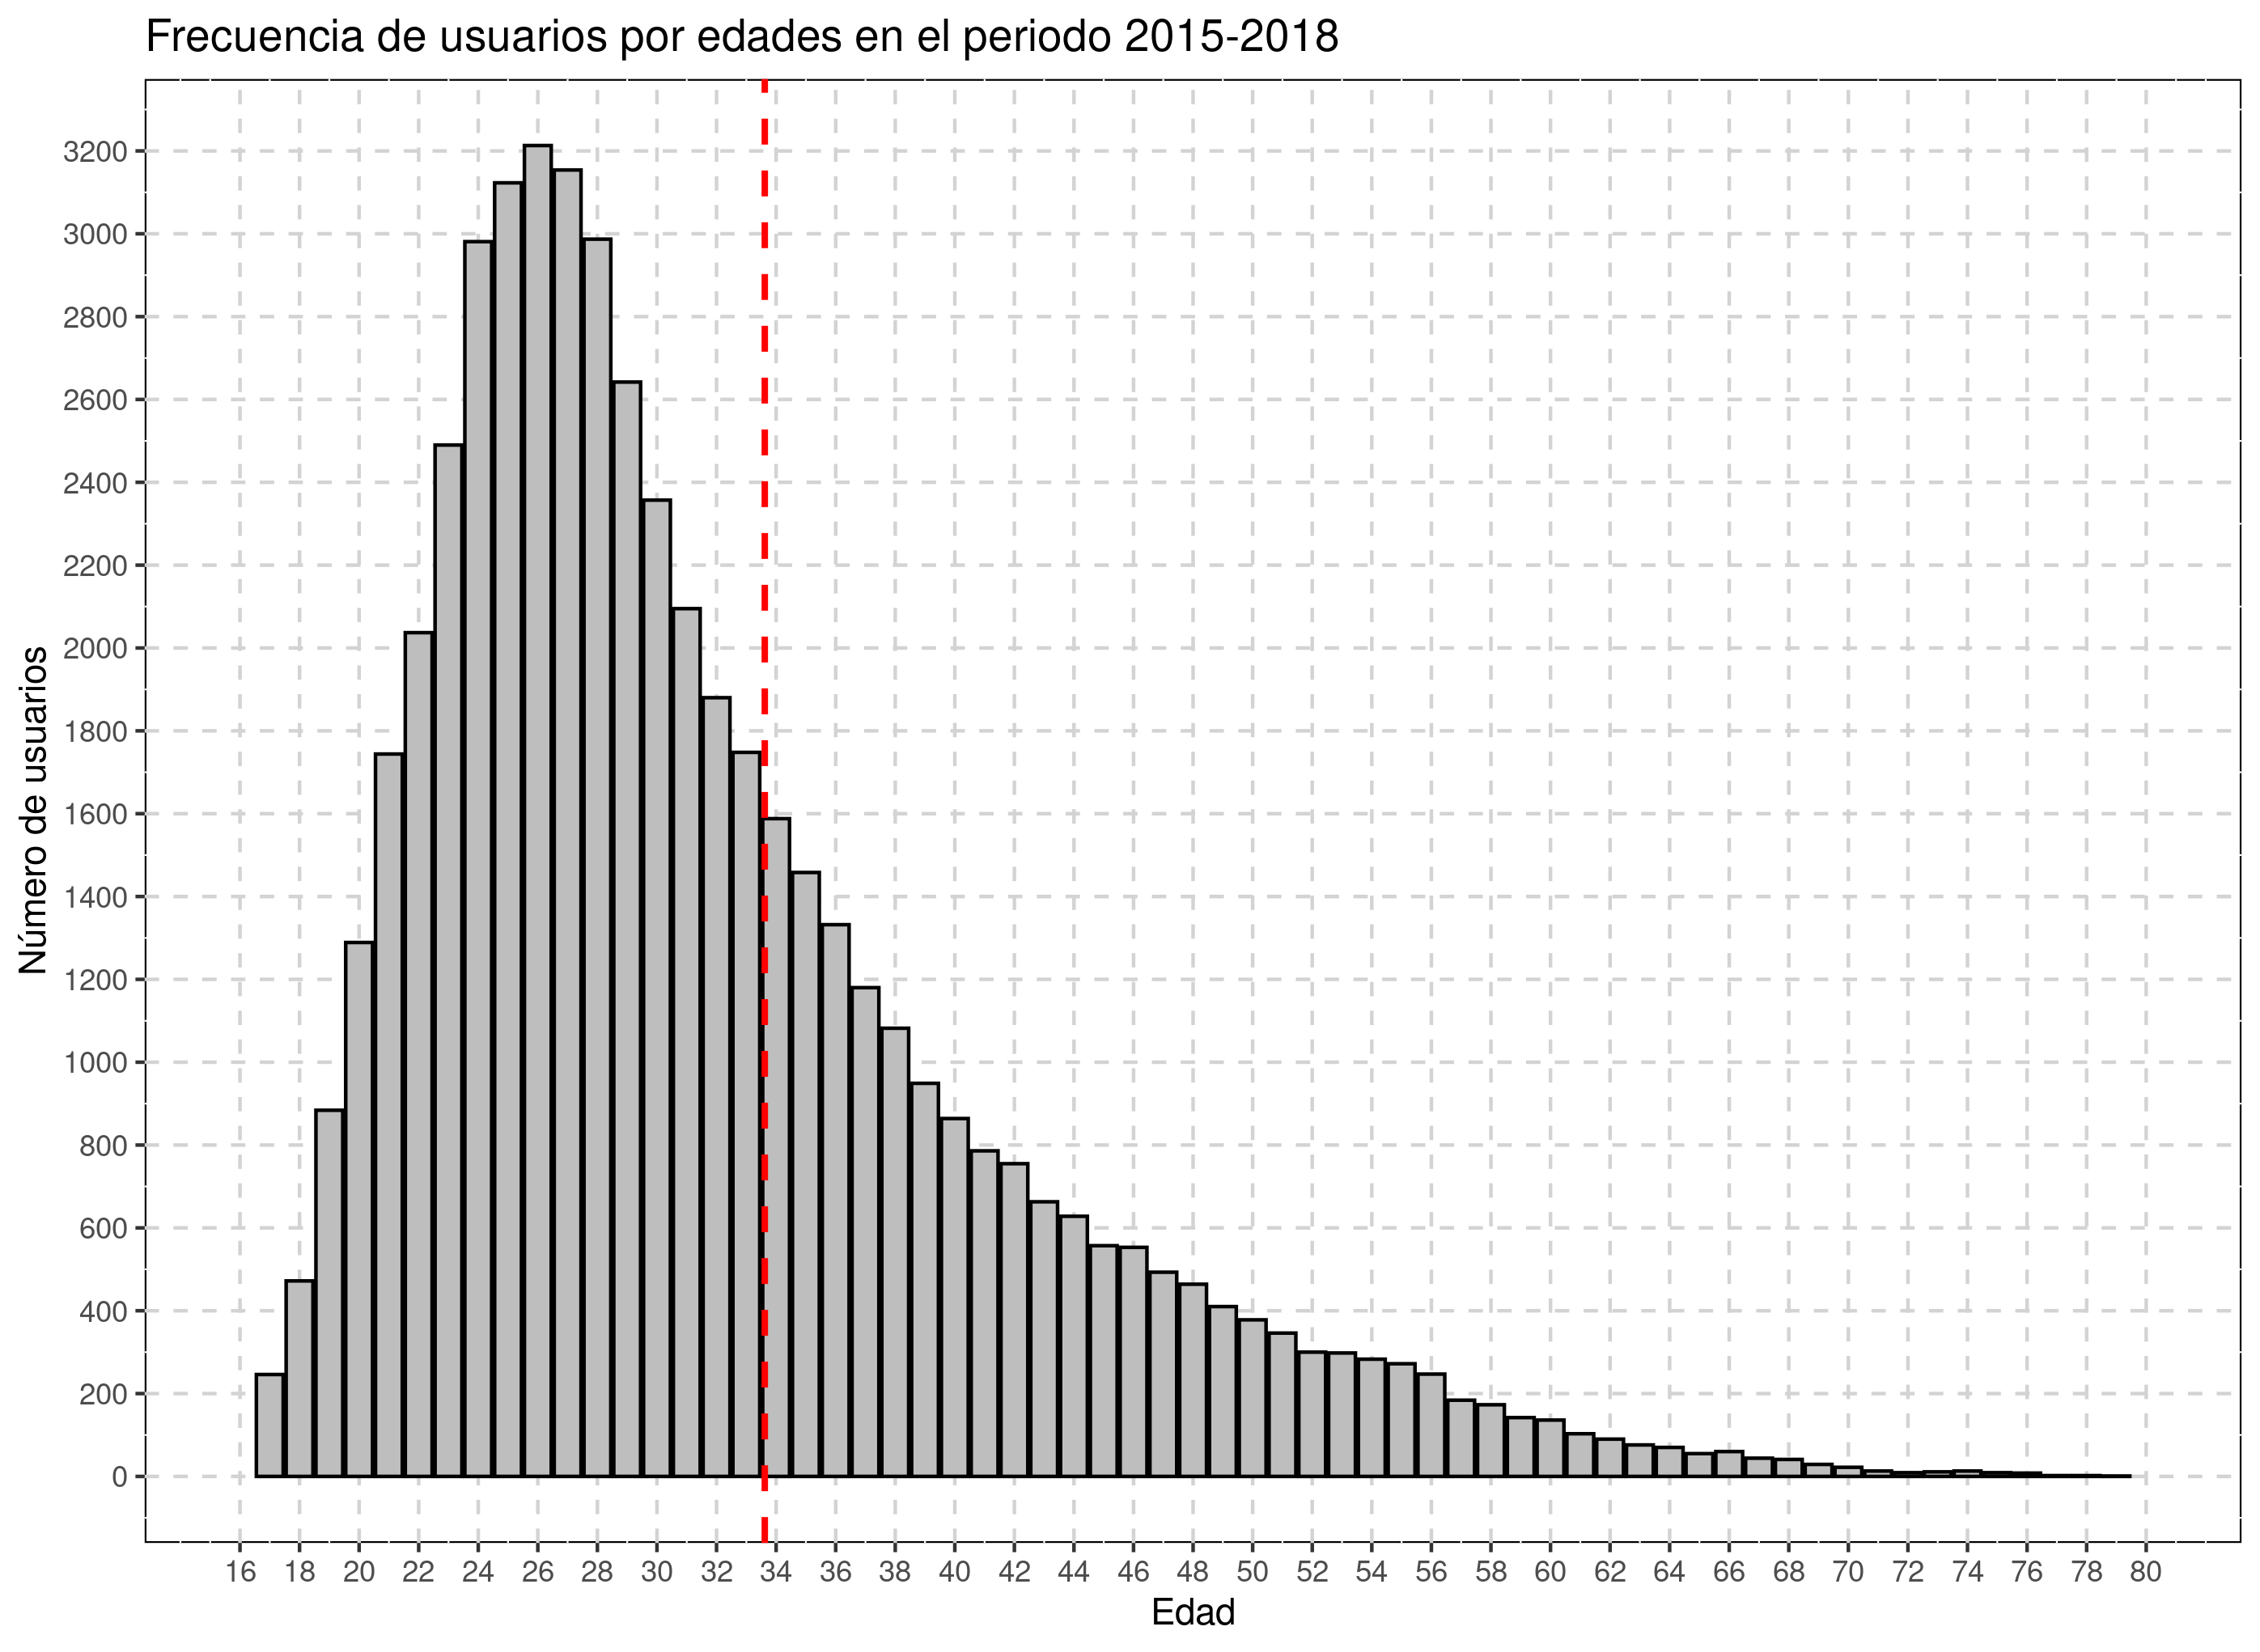
\includegraphics[width=14cm]{Graphics/age_distribution}
	\caption{Distribución de usuarios por edad en el periodo de 2015 a 2018.}
	\label{fig:agedistribution}
\end{figure}

Uno de los requisitos para poder adquirir una suscripción al sistema MiBici es ser mayor de 16 años, y en caso de ser menor de edad, ser acompañado por un padre o tutor. Es por esto que la edad mínima registrada es de 16 años.
\par Si separamos a los usuarios por género, las distribuciones de edades serían como en la figura \ref{fig:agegenderdistribution}. En donde se puede observar que para ambos géneros, se tiene una distribución similar.

\begin{figure}[H]
	\centering
	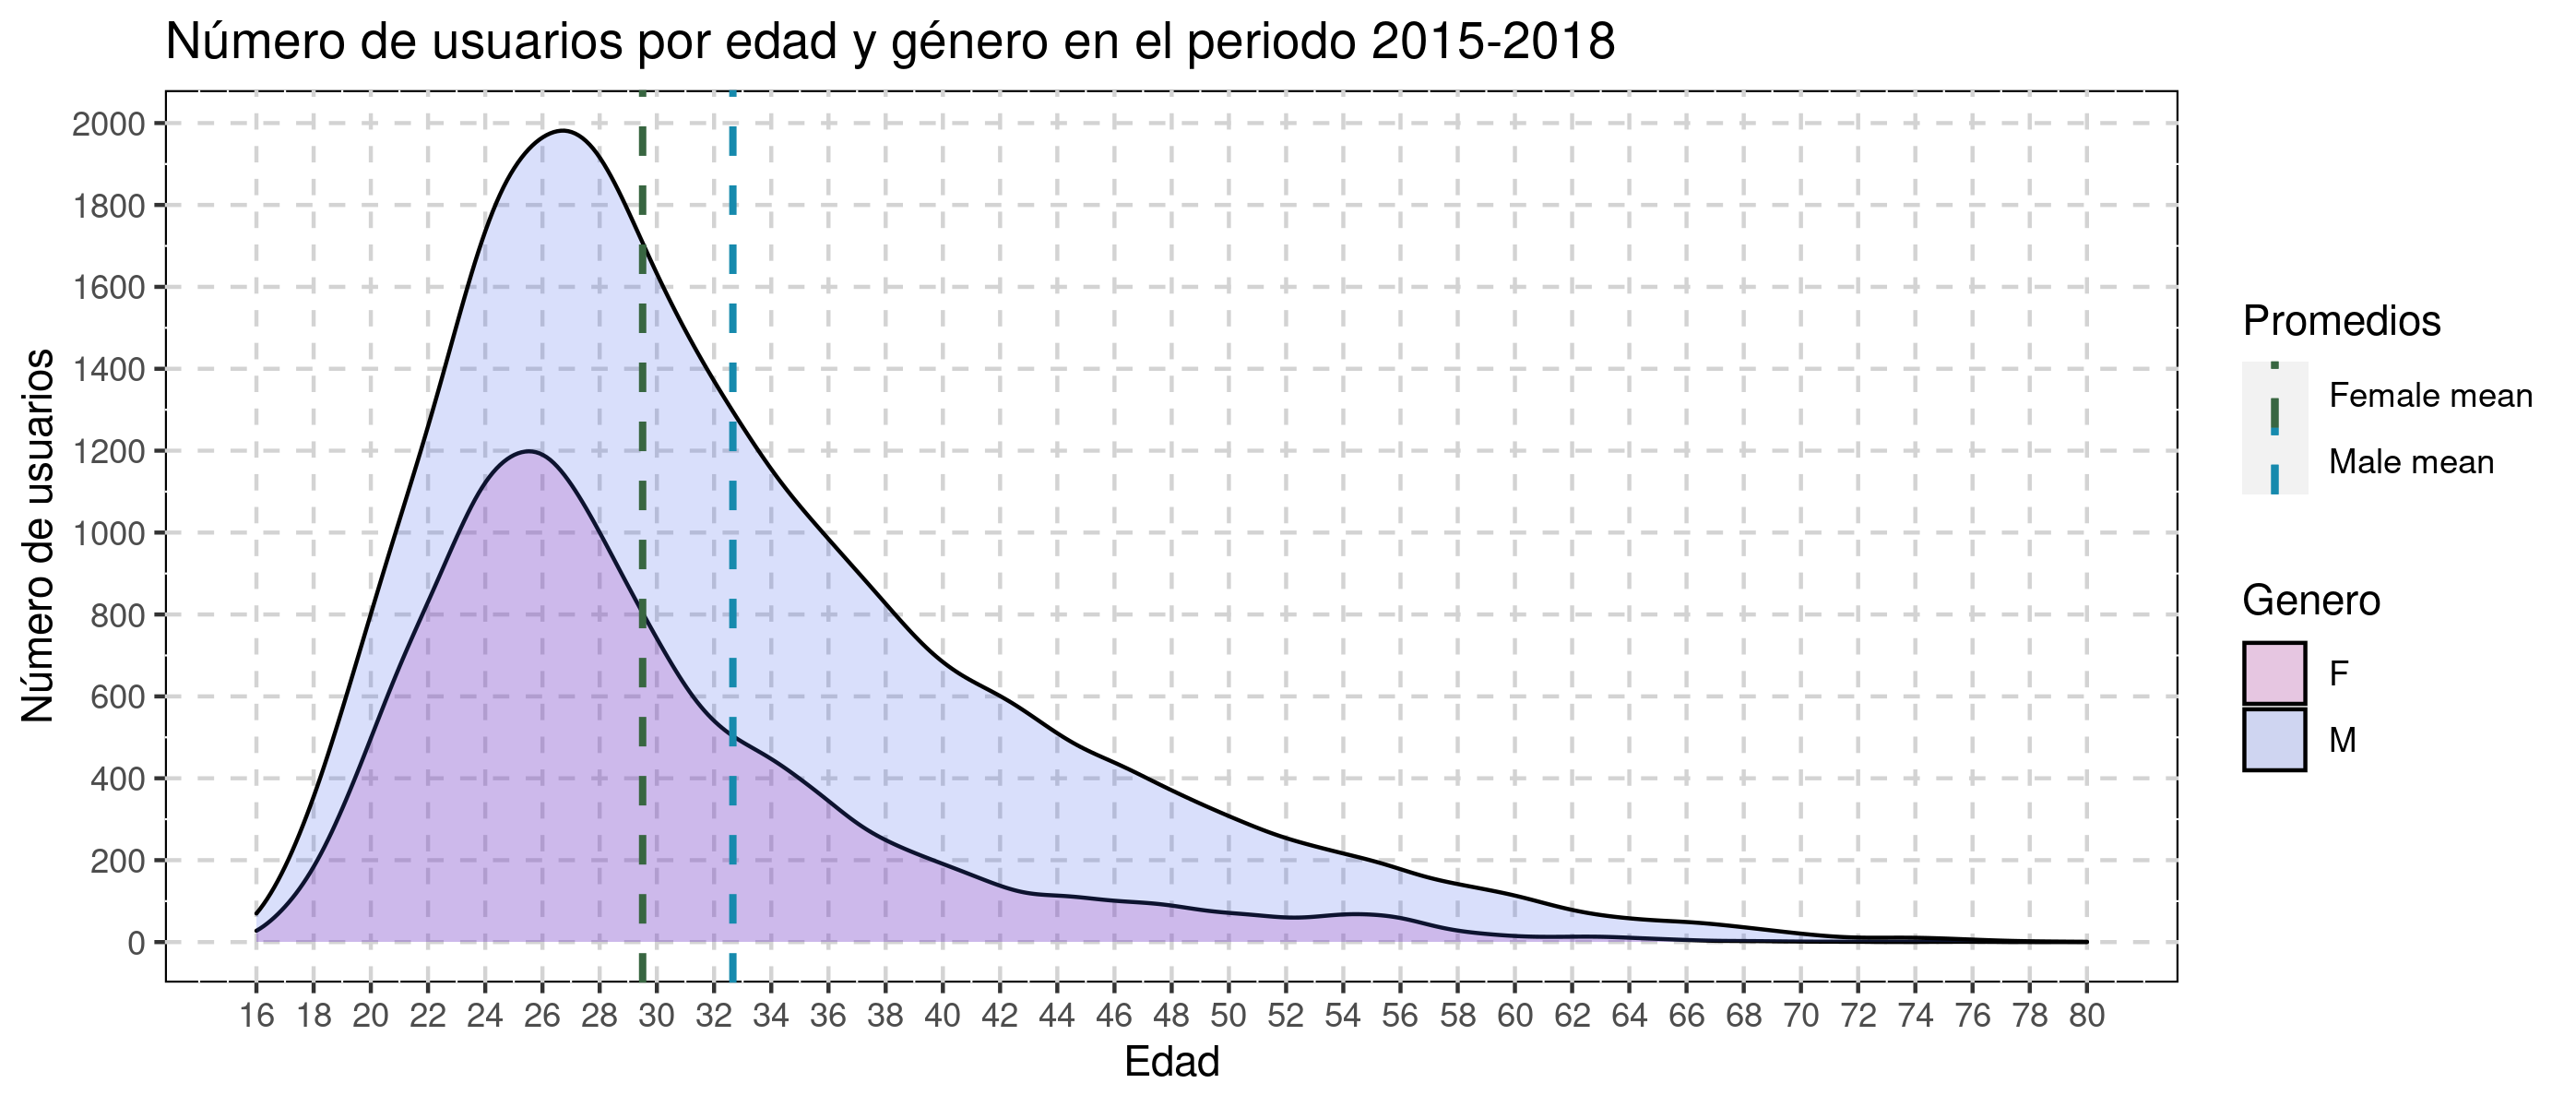
\includegraphics[width=14cm]{Graphics/age_gender_distribution}
	\caption{Distribución de edad de los usuarios, separados por género en el periodo de 2015 a 2018.}
	\label{fig:agegenderdistribution}
\end{figure}

En las figuras \ref{fig:agegenderdistribution} y \ref{fig:genderprop} se puede notar que el número de usuarios de género masculino es mayor que los de género femenino, además, es posible ver que hay una diferencia en la edad promedio de los usuarios de cada género. Siendo la media de la edad para el género femenino de $29.50$ años y para el género masculino de $32.66$ años.